\documentclass[11pt, oneside]{article}   	% use "amsart" instead of "article" for AMSLaTeX format
\usepackage{geometry}                		% See geometry.pdf to learn the layout options. There are lots.
\geometry{letterpaper}                   		% ... or a4paper or a5paper or ... 
%\geometry{landscape}                		% Activate for for rotated page geometry
%\usepackage[parfill]{parskip}    		% Activate to begin paragraphs with an empty line rather than an indent
\usepackage{graphicx}				% Use pdf, png, jpg, or eps§ with pdflatex; use eps in DVI mode
								% TeX will automatically convert eps --> pdf in pdflatex		
\usepackage{amssymb}
\usepackage{amsmath}
\usepackage{parskip}
\usepackage{color}
\usepackage{hyperref}

\title{Your title here}
%\author{The Author}
%\section{}
%\subsection*{}
\date{}							% Activate to display a given date or no date

\graphicspath{{/Users/telliott_admin/Dropbox/Tex/png/}}
% \begin{center} 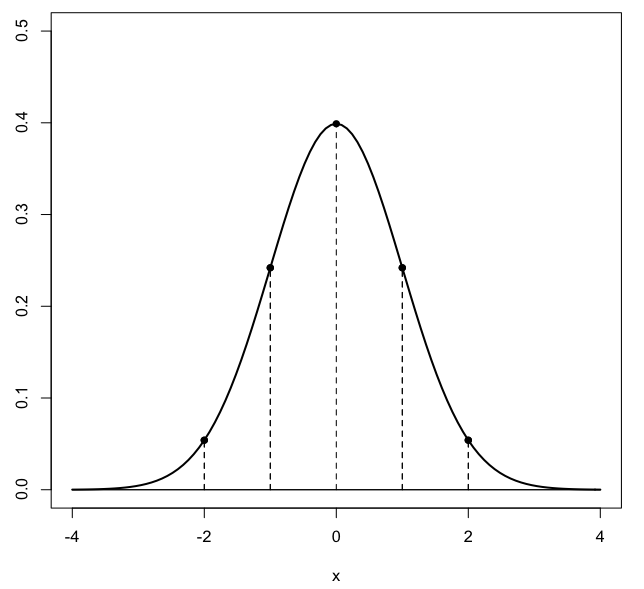
\includegraphics [scale=0.4] {gauss3.png} \end{center}

\begin{document}
\maketitle
\Large
\subsection*{vector fields}
A vector field assigns to every point $(x,y)$ in a region $R$ in the plane a vector $\mathbf{F}(x,y)$ with two components
\[ \mathbf{F}(x,y) = M(x,y) \mathbf{i} + N(x,y) \mathbf{i} \]
Each of the component functions $M$ and $N$ takes an ordered pair of real numbers and outputs a real number.  As a shorthand, we could write:
\[ \mathbf{F} = \langle M, N \rangle \]
In three dimensions we might have $\mathbf{F} = \langle M, N, P \rangle $ or $\langle P, Q, R \rangle$.  We could also write the components of $\mathbf{F}$ explicitly as some functions of $x$ and $y$, e.g.
\[ \mathbf{R} = \langle x,y \rangle \]
This is the field of radial vectors, all of which point in the direction opposite to the origin, and have length $r = \sqrt{x^2 + r^2}$.  We could also normalize to get $\mathbf{R}/r$ or even $\mathbf{R}/r^2$.

The spin field is $\mathbf{S} = \langle -y,x \rangle$.  These can be normalized or divided by $r^2$ as for $\mathbf{R}$.

A \emph{gradient field} is the gradient of some function $f$ which is called the potential.  Such fields are conservative, as we'll see later on.  Recall that the gradient is
\[ \nabla f = \langle f_x, f_y \rangle \]
where by $f_x$ I mean the $x$-derivative of $f$.  The radial fields are all gradient fields.  Consider
\[ f(x,y) = \frac{1}{2}(x^2 + y^2) \]
Clearly
\[ \nabla f = \langle x, y \rangle = \mathbf{R} \]
The gradient is everywhere perpendicular to the level curves $f(x,y) = c$.

Some fields are gradient fields, and some are not.

What is the potential function for 
\[ \frac{\mathbf{R}}{r} = \frac{1}{\sqrt{x^2 + y^2}} \  \langle x,y \rangle \]

What function $f$ has as its $x$-derivative $x/\sqrt{x^2 + y^2}$?
\[ \frac{\partial}{\partial x} \  \sqrt{x^2 + y^2} =  \ ?\]
That looks right.



\end{document} 